% update for ECCV'14 by Michael Stark and Mario Fritz
% updated in April 2002 by Antje Endemann
% Based on CVPR 07 and LNCS, with modifications by DAF, AZ and elle, 2008 and AA, 2010, and CC, 2011; TT, 2014

\documentclass[runningheads]{llncs}
\usepackage{graphicx}
\usepackage{amsmath,amssymb} % define this before the line numbering.
\usepackage{color}
\usepackage[width=122mm,left=12mm,paperwidth=146mm,height=193mm,top=12mm,paperheight=217mm]{geometry}
%\usepackage{ruler}
\usepackage{array}
\usepackage{float}
\usepackage{subfig,caption}
\usepackage{lipsum}
\usepackage{comment}
\renewcommand{\arraystretch}{1.1}

\begin{document}
% \renewcommand\thelinenumber{\color[rgb]{0.2,0.5,0.8}\normalfont\sffamily\scriptsize\arabic{linenumber}\color[rgb]{0,0,0}}
% \renewcommand\makeLineNumber {\hss\thelinenumber\ \hspace{6mm} \rlap{\hskip\textwidth\ \hspace{6.5mm}\thelinenumber}}
% \linenumbers
\pagestyle{headings}
\mainmatter
\title{Analyzing The Performance of Multilayer Neural Networks for Object Recognition} % Replace with your title

\titlerunning{Analyzing The Performance of Multilayer Neural Networks for Object Recognition}

\authorrunning{Pulkit Agrawal, Ross Girshick, Jitendra Malik}

\author{Pulkit Agrawal, Ross Girshick, Jitendra Malik \\ \{pulkitag, rbg, malik\}$@$eecs.berkeley.edu}
\institute{University of California Berkeley}


\maketitle

\begin{abstract}
In 2012 Krizhevsky et al. demonstrated that a Convolutional Neural Network (CNN) trained on large amount of data as part of the ImageNet challenge significantly outperformed traditional computer vision approaches on image classification. Subsequently, Girshick et al. (2013) exploited these features to establish the new state of the art on PASCAL object detection. This suggests that computer vision is undergoing a feature revolution akin to that following SIFT and HOG nearly a decade ago. It is therefore important to get more insights into features learned by these networks. Our paper provides answer to the following four questions: (a)What happens during finetuning of a discriminatively pretrained network? (b)How much information is in the location and how much of it is in the magnitude of filter activation? (c)Does a multilayer CNN contain Grand-Mother Cells? (d)How does training of CNN progress over time?
\dots
\keywords{We would like to encourage you to list your keywords within
the abstract section}
\end{abstract}

\section{Introduction}
The breakthrough work of \cite{Kriz} created a splash in the computer vision community by presenting a convolutional neural network (CNN) model which easily surpassed all existing methods on the ImageNet ILSVRC-2012 image classification challenge \cite{imagenet}.  The top-5 error rates dropped by an exceptional amount to 16.4\% from  26.2 \% (achieved by the second best alternative.) At that time, it was unclear if these networks would be useful for other computer vision tasks. A few months later, \cite{Decaf} demonstrated that features learnt by such networks generalize and achieve state of the art results on image classification challenges such as SUN-397\cite{sun}, Caltech-UCSD Birds and Caltech-101. 

More recently, features extracted using CNNs were used to achieve impressive results on object detection (RCNN \cite{Rcnn}) which dwarf the existing state of art by a big margin. \cite{Rcnn} achieved a mAP of 54.1 v/s 41.7 achieved by \cite{regionlets} on the PASCAL VOC 2007 detection challenge. Given that over the last few years, negligible progress was made on various PASCAL VOC challenges, these results are significant and strongly suggest that we might be in the middle of a feature revolution akin to the one ushered by introduction of HOG \cite{Hog} and SIFT \cite{Sift} in the mid 2000s.  

It is not the first time that CNN have generated great interest within the computer vision community. In late eighties LeNet\cite{Lecun89} achieved state of art performance on the task of MNIST digit classification. However, by late nineties interest in neural networks started to wane. One major reason was that a large number of parameters such as the number of layers, number of units in each layer, the learning rate needed to be manually set in order to successfully train these networks. Support Vector Machines (SVMs) on the other hand provided an easy alternative for achieving the same performance levels with only one parameter (C) to tune. Presently, given the impressive performance of CNN \cite{Kriz, Decaf, Rcnn} - the stage is all set for their second renaissance in mainstream computer vision. 

We take the view that rich feature hierarchies provided by CNN are very likely to emerge as the prominent feature extractor for computer vision models over the next few years. Feature extractors such as SIFT and HOG afford an intuitive interpretation of templates composed of oriented edge filters. However, we have little understanding of what visual features do the different layers of a CNN encode and what is the best way of using this information. We believe that developing such an understanding is an interesting scientific pursuit and an essential exercise prior to designing computer vision methods which can optimally use these features.

In this paper we address some of these issues through an empirical scientific investigation of multilayer CNNs. We characterize the features obtained from different layers by first teasing apart the importance of the magnitude and location of filter responses (sec \ref{sec-where-info}). We report that CNNs naturally provide sparse binary features and that for image classification the location of filter responses in the intermediate layers is not critical. Further, we establish an objective methodology for studying the question of how distributed are the feature representations and whether there are Grandmother Cell (\cite{Barlow, Grandmother}) like filters in the CNN  (sec \ref{sec:grand-mother}. We find that feature representations are distributed and only for a few classes the CNN develops Grandmother Cell like filters.  

Proponents of multilayer networks have argued in the past that unsupervised pre-training followed by finetuning is helpful for learning features which improve performance on discriminative tasks such as image classification \cite{GoogleCat, DeepPre, HintonPre}. Finetuning a network is the process of slowly updating pre-learned parameters to minimize a target loss function for a new task at hand. Since, multilayer networks consist of a large number of parameters they are prone to overfitting when trained on small datasets. Instead of unsupervised pre-training, \cite{Decaf, Rcnn} have made a strong case for learning features using discriminative pre-training followed by finetuning for a specific task at hand. They first trained a network for the task of image classification on Imagenet and then finetuned the network for object detection on PASCAL. In this work, we analyse the effect of finetuning on different layers of a CNN (section \ref{sec:fine}). We find that for moderately sized datasets (upto $\sim$ 50K images), finetuning only effects the top two fully connected layers (section \ref{sub:net-arch}) whereas the lower convolutional layers are mostly unchanged. We show that this observation can be used to make finetuning 2x faster with negligible effect on performance. We also demonstrate that a network can be trained from scratch using data only from the PASCAL dataset to achieve the state of art performance on object detection reported by \cite{Rcnn}. Further, by simply using more data for finetuning, we report a $10\%$ increase in performance for object detection over \cite{Rcnn}. 

Finetuning can also be viewed as a method for transfer learning (NEED REF for transfer learning). It is interesting to draw a parallel between this and the way we humans learn. As children, we can easily learn new things but as we grow older it becomes harder. Similarly, it is possible that if CNNs are pretrained for too long, it becomes harder to generalize to a new task. In other words, pre-training can lead to overfitting and consequently lead to worse performance on a new task due to dataset bias \cite{datasetBias}. Thus, we are faced with the question - is there an optimal time for which pre-training should be carried out? Rather surprisingly, we find that fitting better to ImageNet allows lower generalization error when moving to other datasets (section \ref{sec:train}), i.e. pre-training more improves performance.

\section{Training Procedure}
\label{sec:train}
\subsection{Network-Architecture and Nomenclature}
\label{sub:net-arch}
We closely followed the CNN architecture proposed in \cite{Kriz} and publically available code of \cite{caffe} for all our experiments. The various layers of the CNN are organized as following: first 2 layers are subdivided into 4 sublayers each - convolution (conv), followed by rectified linear units (relu), pooling (pool) and contrast normalization (norm). Layers 3, 4 are composed of conv units followed by relu units. Layer 5 consists of conv units, followed by relu and pool units. The last two layers are fully connected (fc). In this work, when we refer to layers 1,2 and 5 we mean the output of pool units and for layers 3,4,6,7 we mean the output of relu units. The imagenet network was trained for 310000 iterations and achieved an error rate of only about 2\% higher on the ILSVRC validation set 2012. \newline
The term ImgNet is used to refer to a CNN trained for Imagenet classification. FT or FT-Net refers to a finetuned network whereas as FC-FT or FC-FT-Net refers to a network finetuned by setting the learning rate of the first 5 layers to zero. We use the terms CNNs and ConvNets interchangeably to refer to multilayer network architectures of the type proposed in \cite{Kriz}. Terms filter/unit are used interchangeably to refer to filters of the CNN and GT-BBOX/gt-bbox stands for Ground truth bounding boxes from the PASCAL-VOC-2007 detection challenge and mAP refers to mean average precision \cite{Pascal}.

\subsection{Training Setup} 
\label{sub:train-setup}
Results for image and GT-BBOX classification were obtained by training linear SVMs on train-val sets of PASCAL-VOC-2007 \cite{Pascal} and tested on the test set. For detection we closely follow the RCNN setup described in \cite{Rcnn}. For SUN-397 \cite{sun} we used a non-standard train-test splits since it was infeasible to finetune CNNs for 10 standard subsets proposed by \cite{sun}. Instead, we randomly split the dataset into 3 parts namely train,val and test using 50\%,10\% and 40\% of the data. The distribution of classes was uniform across all the 3 sets. Results on these splits are only used to support investigations into properties of CNNs and not for comparing against other scene-classification methods.  
 
\subsubsection{Fine-Tuning}
\label{sub:fine-train}
CNN were finetuned using SGD (Stochastic Gradient) with a starting learning rate set to $\frac{1}{10}^{th}$ of the initial learning rate used for training the network for Imagenet classification. This choice was made to prevent overfitting of CNNs to the new task for which the network was finetuned for. At every 20,000 iterations learning rate was reduced by a factor of 10 and mini-batch size of 128 was used. We closely followed \cite{Rcnn} for finetuning CNNs for object detection. 

\subsection{Method of Entropy Computation}
\label{sub:def-ent}
We define the entropy of a filter with respect to a given set of image-label pairs in the following way. Each image, when passed through the convolutional neural network produces a $p \times p$ heatmap of filter responses. (e.g. p = 6, for a layer 5 filter). We vectorize this heatmap into a vector of scores of length $p^2$ and with each element of this vector we associate the class label of the image. Thus, for each image we have a score vector and a label vector of length $p^2$ each. Next, we concatenate score vectors and label vectors from N images into a giant score vector and a giant label vector  of size $Np^2$ each. Now for every score threshold we consider all the labels which have an associated score $\geq$ to this threshold score. The entropy of this set of labels is the entropy of the filter at this threshold. As this threshold changes, entropy traces out a curve which we call as the entropy curve.  


\section{How much information is in the magnitude and the location of filter responses?}
\label{sec-where-info}
For studying the importance of location and the magnitude of filter responses, we constructed a set of ablations (described in fig \ref{fig:features}) and the studied their effect under the experimental conditions of image classification (see table \ref{table:class-ablation}) and object detection (see table\ref{table:det-ablation}).

\begin{figure}[t!]
\centering
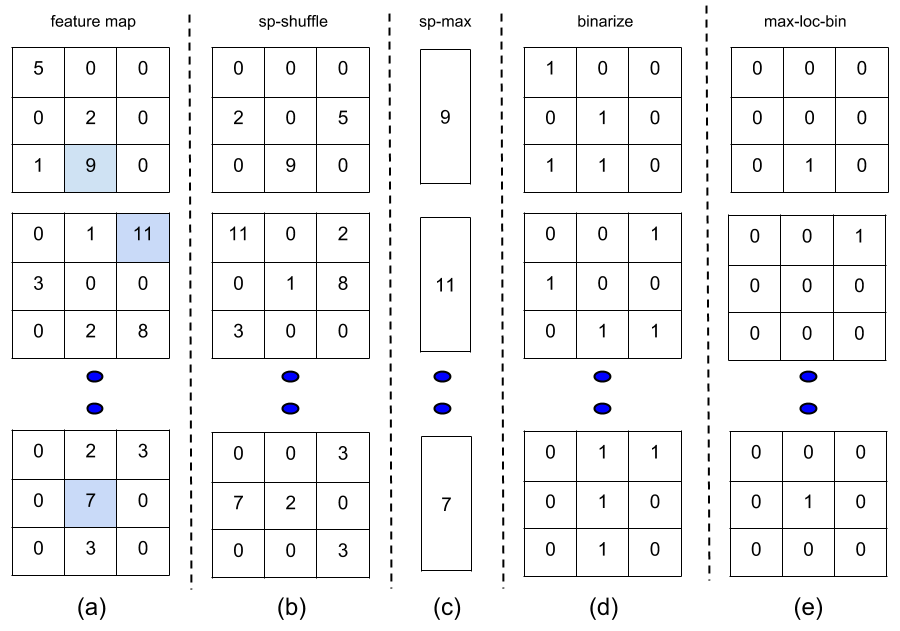
\includegraphics[height=6.5cm]{images/features1.png}
\caption{(a) For illustration, consider the output of a hypothetical layer of size k*k*N (k=3 for convolutional layers and k=1 for FC layers), which has N filters and their responses at k*k spatial locations. Linear SVMs were trained (one for each layer) after vectorizing (i.e. x(:) in matlab) features into a one-dimensional vector of length k*k*N to measure performance of different layers. Next, feature ablations as described below were applied before training SVMs and performance was compared against the un-ablated features. The set of k*k locations for each filter is called its feature map. (b) \textit{spatial-shuffle}(sp-shuffle) -  A random permutation is applied to the set of k*k activations associated with each feature map. Different images see different permutations. (c)\textit{spatial max}(sp-max): For each feature map, the maximum value is selected from the set of k*k activations. (d)\textit{binarization}(bin) Feature dimensions with value $>0$ are set to 1 and others to 0.}
\label{fig:features}
\end{figure}

\subsection{How important is the magnitude of activation ?}
\label{sub:imp-mag}
\setlength{\tabcolsep}{2pt}
\begin{table}[t!]
\begin{center}
\caption{Percentage non-zeros (sparsity) in features of various layers of CNN.}
\label{table:sparse}
\scalebox{1}{
\begin{tabular}{|c|c|c|c|c|c|c|}
\hline
conv-1 & conv-2 & conv-3 & conv-4 & conv-5 & fc-6 & fc-7 \\
\hline
$87.5 \pm 4.4$ & $44.5 \pm 4.4$ & $31.8 \pm 2.4$ & $32.0 \pm 2.7$ & $27.7 \pm 5.0$ & $16.1 \pm 3.0$ & $21.6 \pm 4.9$ \\
\hline
\end{tabular}}
\end{center}
\end{table}
\setlength{\tabcolsep}{1.4pt}

Binarization leads to loss of information contained in the magnitude of filter responses. We report that this leads to negligible decline in performance for both classification and detection (tables \ref{table:class-ablation}, \ref{table:det-ablation}). Further, the sparsity of CaffeNet features are reported in table \ref{table:sparse}. Notice, that the fc layers are quite sparse. A lot of work in image retrieval (NEED REF) focuses on finding sparse binary features - and our results indicate that one can get these `for free' from CNN features. 

\subsection{How important is where a filter activates?}
\label{sub:imp-loc}
The \textit{sp-max} and \textit{sp-shuffle} are two ablations which devoid the feature vector of the location of the filter response. For image classification, these lead to a large difference in performance between original and ablated conv-1 features, but gradually decreasing difference for higher layers (table \ref{table:class-ablation}). Infact, the performance of conv-5 after \textit{sp-max} is close to the original performance. This indicates, that a lot of information important for classification is encoded in the activation of the filters and not necessarily in the pattern of their activations. However, for detection \textit{sp-max} (tables \ref{table:det-ablation}) leads to a large drop in performance. 
This may not be surprising as in contrast to classification, for detection we need precise localization.

\setlength{\tabcolsep}{4pt}
\begin{table}[t!]
\begin{center}
\caption{Ablation study on PASCAL Image Classification (see fig \ref{fig:features})}
\label{table:class-ablation}
\begin{tabular}{lccccc}
\hline\noalign{\smallskip}
layer & no-ablation & bin & sp-shuffle & sp-max & sp-max-bin \\
\noalign{\smallskip}
\hline
\noalign{\smallskip}
conv-1 & $25.1 \pm 0.5$ & $17.7 \pm 0.2$ & $15.1 \pm 0.3$ & $25.4 \pm 0.5$ & $8.3  \pm 0.2$  \\ 
conv-2 & $45.3 \pm 0.5$ & $43.0 \pm 0.6$ & $32.9 \pm 0.7$ & $40.1 \pm 0.3$ & $11.7 \pm 0.3$  \\ 
conv-3 & $50.7 \pm 0.6$ & $47.2 \pm 0.6$ & $41.0 \pm 0.8$ & $54.1 \pm 0.5$ & $12.3 \pm 0.3$ \\
conv-4 & $54.5 \pm 0.7$ & $51.5 \pm 0.7$ & $45.2 \pm 0.8$ & $57.0 \pm 0.5$ & $11.3 \pm 0.2$  \\
conv-5 & $65.6 \pm 0.6$ & $60.8 \pm 0.7$ & $59.5 \pm 0.4$ & $62.5 \pm 0.6$ & $28.0 \pm 0.3$ \\
fc-6   & $71.7 \pm 0.3$ & $71.5 \pm 0.4$ &  -             &  -        &  -    \\
fc-7   & $74.1 \pm 0.3$ & $73.7 \pm 0.4$ &  -             &  -        &  -   \\
\hline
\end{tabular}
\end{center}
\end{table}
\setlength{\tabcolsep}{1.4pt}

\setlength{\tabcolsep}{1pt}
\begin{table}[t!]
\begin{center}
\caption{Ablation study on PASCAL Object Detection using conv-5 features\cite{Rcnn}. Binarization leads to negligible drop in performance whereas as \textit{sp-max} causes a large drop in performance.}
\label{table:det-ablation}
\scalebox{0.70}{
\begin{tabular}{l|cccccccccccccccccccc||c}
\hline\noalign{\smallskip}
Feature & aero & bike & bird & boat & bottle & bus & car & cat & chair & cow & table & dog & horse & mbike & person & plant & sheep & sofa & train & tv & mAP \\
\noalign{\smallskip}
\hline
conv-5  & 57.8 & 63.9 & 38.8 & 28.0 & 29.0 & 54.8 & 66.9 & 51.3 & 30.5 & 52.1 & 45.2 & 43.2 & 57.3 & 58.8 & 46.0 & 27.2 & 51.2 & 39.3 & 53.3 & 56.6 & 47.6 \\
bin & 57.9 & 61.3 & 32.6 & 24.7 & 27.5 & 55.0 & 64.7 & 49.8 & 25.3 & 47.4 & 44.5 & 40.3 & 54.6 & 56.4 & 43.6 & 27.1 & 48.4 & 41.6 & 54.3 & 57.6 & 45.7 \\
sp-max & 35.0 & 38.7 & 17.3 & 16.9 & 13.9 & 38.4 & 45.6 & 29.2 & 11.0 & 20.2 & 21.0 & 23.5 & 27.2 & 37.0 & 20.5 & 7.0 & 30.3 & 13.4 & 28.3 & 32.9 & 25.4 \\
\noalign{\smallskip}
\hline
\end{tabular}}
\end{center}
\end{table}
\setlength{\tabcolsep}{1.4pt}


\subsection{Discussion}
For classification although sp-max and binarization by themselves are not detrimental - their combination (sp-max-bin) is catastrophic to performance.

\section{Are there Grand-Mother Cells in CNNs? How distributed are the representations?}
\label{sec:grand-mother}
 

\cite{GoogleCat} showed the emergence of cat and people specific filters in a deep non-convolutional network. More recently,\cite{DeConv}, \cite{Simonyan} presented visualization methods to find the optimal visual input for a single filter. However, these methods implicitly assumed the presence of single filters which are class specific. This may not be true. Also, visualization methods do not convey the full story. In particular, finding the  optimal visual pattern for a specific filter is akin to maximising,  They are subjective and it is unclear what conclusions may be drawn. Visualizing the tuning of a few filters tells us very little about what the other filters might be doing. To the best of our knowledge there is little work which tries to find an objective answer to this question.

In neuroscience, the presence of neurons  has been hotly debated Most of the above mentioned work can be mathematically treated either as estimating Prob(Filter Activity$\geq$ thresh $|$ Class) or finding the optimal stimulus for a specific unit. We argue that this by itself is an incomplete metric for interpreting how selective a certain filter is. (A hypothetical filter which has the same activation for all classes will score high on this measure.)  The right metric to evaluate if a certain filter is very selective (aka Grand-Mother Cell \cite{Barlow}) is precision defined as Prob(Class $|$Filter Activity $\geq$thresh)

We divide our analysis into two parts. In sec \ref{sub:class-specific-unit} we try to address if there exist filters with very high precision (aka Grand-Mother cells) and in sec \ref{sub:how-many} we answer how many filters are required to discriminate a class. 

\subsection{Are there high precision filters in layer 5?}
\label{sub:class-specific-unit}
Precision for each filter from layer 5 is computed in a way analogous to entropy computation described in \ref{sub:def-ent}. In the final step instead of computing the entropy, we compute Prob(Class $|$ Filter Activity $\geq$ threshold). We define the selectivity of a filter as the area under the precision curve. For this computation we use ground truth bounding boxes taken from PASCAL VOC-2007 test challenge.
From figure \ref{fig:prob-sel} it is clear that for some classes such persons and bicycles there are indeed some very high precision filters, but for a lot of classes like sofa and horses no such filters exist. 

\begin{figure}[t!]
\centering
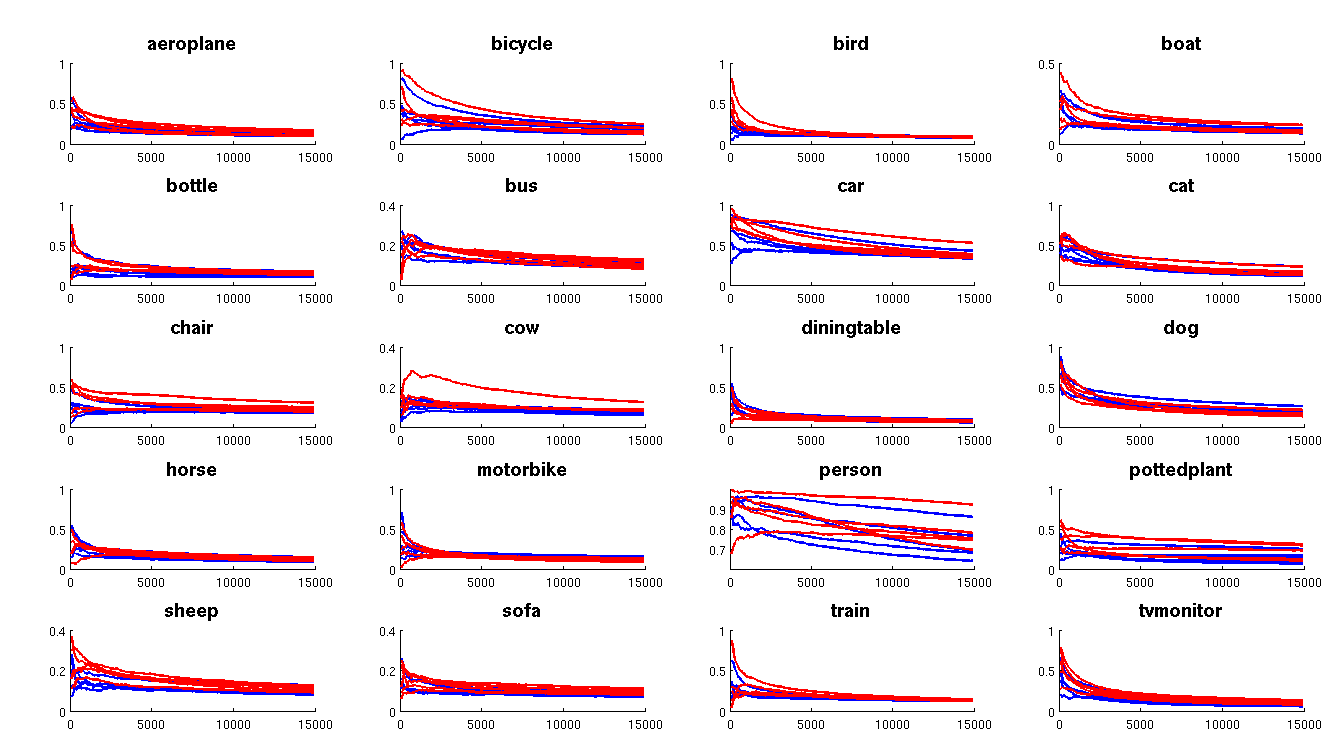
\includegraphics[scale=0.20]{images/prob_sel_dims_top5.png}
\caption{This plot shows the precision curve for the top 5 most selective filters taken from Alex-Net (Blue) and FT-Net(Red) for all PASCAL classes. Y-axis is the precision and X-axis is number of examples.}
\label{fig:prob-sel}
\end{figure}

\subsection{How many filters are required for discrimination?}
\label{sub:how-many}
In order to answer this question we train linear a svm for each class using only a subset of 256 pool-5 filters. In particular we construct subsets of size k, where k takes the values - [1,2,3,5,10,15,20,25,30,35,40,45, \newline 50,80, 100,128,256]. A subset of size k is constructed independently for each class using a greedy selection strategy described in figure \ref{fig:sel-strategy}. We use the variation in performance with the number of filters needed as a metric to evaluate how many filters are needed for each class. 
  
\begin{figure}[t!]
\centering
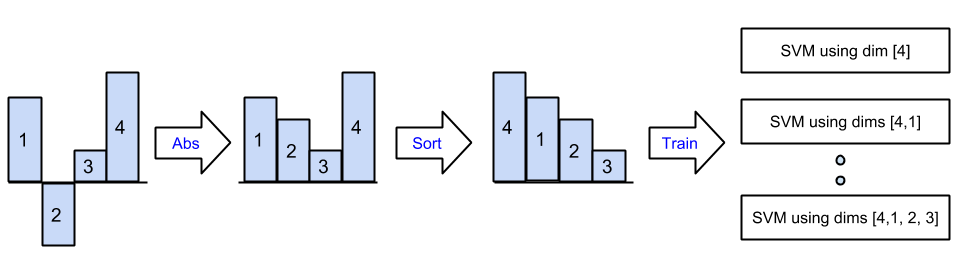
\includegraphics[scale=0.30]{images/how-many.png}
\caption{Illustration of our greedy strategy for constructing subsets of filters. For each class we first train a linear-svm using the spatial-max feature transformation described in section \ref{sub:imp-loc}. Spatial-max leaves us with a 256-D vector wherein each dimension has a one to one correspondence with 256 pool-5 filters. We use the magnitude of each dimension of the learnt weight vector as a proxy for the importance of that dimension towards discriminating a given class. For the purpose of illustration we describe the procedure with a 4-D weight vector shown on the extreme left (the numbers on each bar are the "dimension"). Firstly, we take the absolute value for each dimension and then sort the dimensions based on this value. Then, we chose the top k filters/dimensions from this ranked list to construct a subset of size k.}
\label{fig:sel-strategy}
\end{figure}

The results of our analysis are summarized in fig \ref{fig:svm-sel-dims} and table \ref{table:num-fil}. For classes such as persons, cars, cats we require a relatively few number of filters, but for most of the classes we need to look at around 30-40 filters to achieve atleast 90\% of the full performance. This also indicates, that for a few classes yes, there are grand-mother kind of neurons but for a lot of classes the representation is distributed. Also, as expected the fine-tuned network requires activations of a fewer numbers of filters to achieve the same performance but this reduction in number of filters is not large. 

\begin{figure}[t!]
\centering
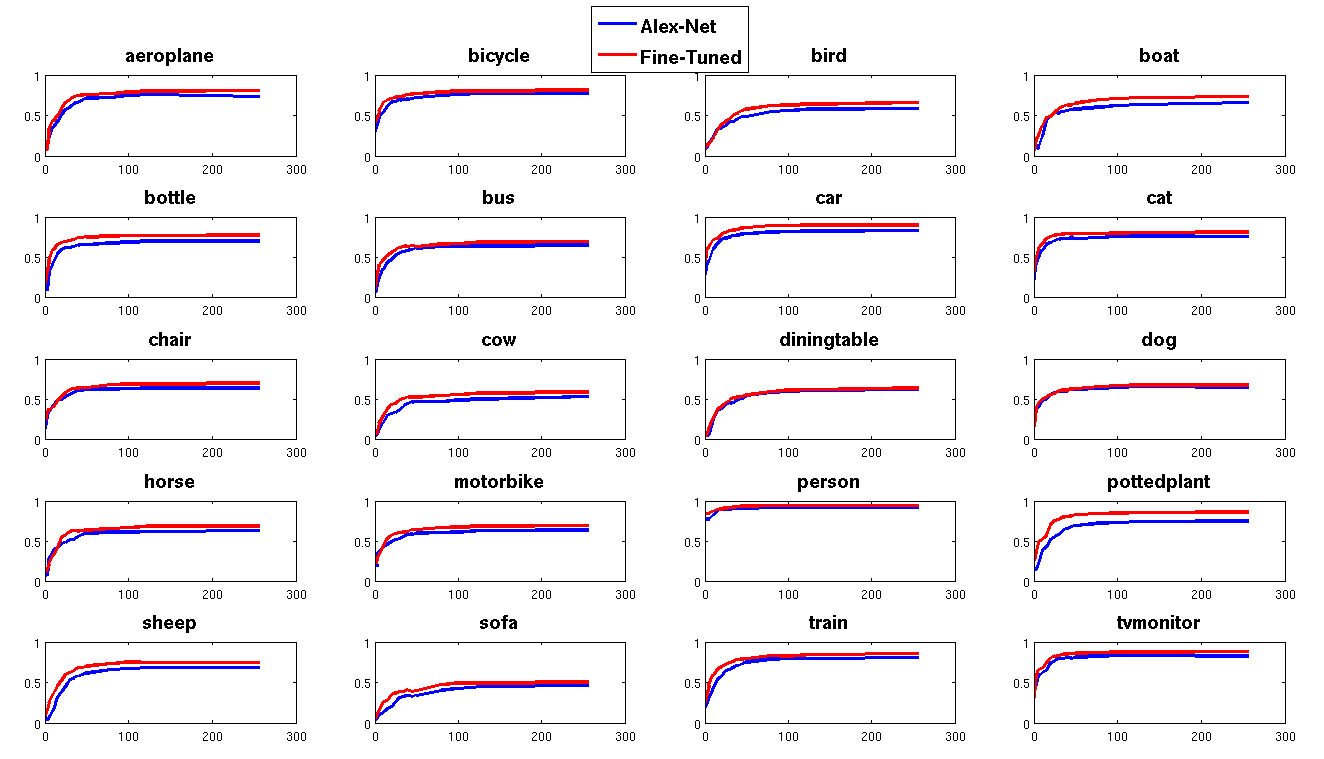
\includegraphics[height=6.5cm]{images/svm_seldims.png}
\caption{Analysis of how many filters are required to classify ground truth bounding boxes for 20 categories taken from PASCAL-2007 detection challenge. The y-axis in each of plot represents classification accuracy measured as mean-ap where as x-axis stand for the number of filters.)}
\label{fig:svm-sel-dims}
\end{figure}



\setlength{\tabcolsep}{1pt}
\begin{table}[t!]
\begin{center}
\caption{Number of filters required to achieve 50\% ,90\% of the full performance for PASCAL classes using Alex-Net(AN) and the Fine-Tuned network(FT)}
\label{table:num-fil}
\tiny
\begin{tabular}{lc||cccccccccccccccccccc}
\hline\noalign{\smallskip}
Net & AP & aero & bike & bird & boat & bottle & bus & car & cat & chair & cow & table & dog & horse & mbike & person & plant & sheep & sofa & train & tv \\
\noalign{\smallskip}
\hline
AN & 50 & 15 & 3 & 15 & 15 & 10 & 10 & 3 & 2 & 5 & 15 & 15 & 2 & 10 & 3 & 1 & 10 & 20 & 25 & 10 & 2 \\ 
FT & 50 & 10 & 1 & 20 & 15 & 5 & 5 & 2 & 2 & 3 & 10 & 15 & 3 & 15 & 10 & 1 & 5 & 15 & 15 & 5 & 2 \\
\hline
\noalign{\smallskip}
AN & 90 & 40 & 35 & 80 & 80 & 35 & 40 & 30 & 20 & 35 & 100 & 80 & 30 & 45 & 40 & 15 & 45 & 50 & 100 & 45 & 25 \\
FT & 90 & 35 & 30 & 80 & 80 & 30 & 35 & 25 & 20 & 35 & 50 & 80 & 35 & 30 & 40 & 10 & 35 & 40 & 80 & 40 & 20 \\
\hline
\end{tabular}
\end{center}
\end{table}
\setlength{\tabcolsep}{1.4pt}

\begin{figure}[t!]
\centering
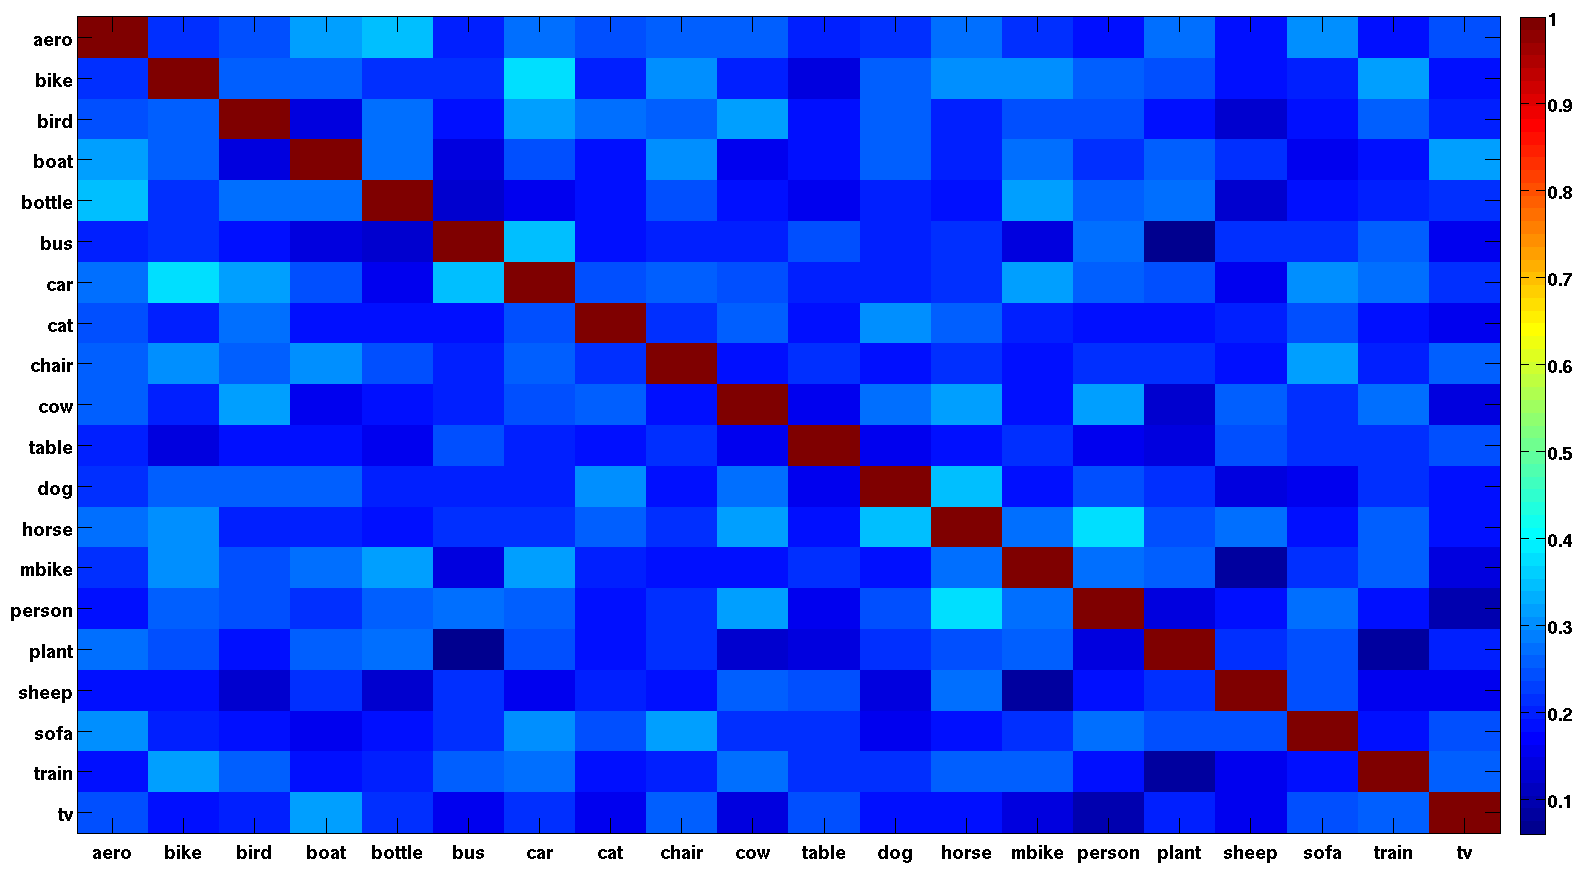
\includegraphics[width=1.0\linewidth]{images/ftNet_commonfilters.png}
\caption{This plot depicts the degree of overlap among the top-50 filters in layer 5 of
finetuned network used for classifying each category of the PASCAL 2007 challenge. Entry
(i,j) of the matrix is the fraction of filters of the i th class which are common with j th class. This plot indicates, that there is very little overlap between filters used for different classes.}
\label{fig:svm-sel-dims}
\end{figure}







\subsection{Discussion}
Although in our analysis we find that for discriminating some classes only a few units suffice whereas for others quite a lot of them are required. The ''extent" to which the code is distributed is likely to be a function of number of filters. If there are a few filters we will expect the code to be more distributed whereas if there are a large number of filters we expect to find more Grandmother kind of cells. The other important tradeoffs to consider are accuracy and training time as a function of number of filters in each layer. We as a community have only had a chance to experiment with a few network architectures out of the exponentially large number of possibilities. Although, it is beyond the scope of the current work determining the optimal number of filters in each layer is an open important question which needs to be addressed! 




\section{What happens when a discriminatively pretrained network is finetuned?}
\label{sec:fine}
Finetuning a network is the process of slowly updating pre-learned parameters to minimize a target loss function for a new task at hand. Since, CNNs consist of large number of parameters they are prone to overfitting when trained on small datasets. Finetuning can be considered as a method of transfer learning and recent results from \cite{Rcnn, Decaf} presented a strong case for this methodology boosting performance. Although, unsupervised pretraining has been widely studied in the multilayer network literature \cite{AmitGeman, DeepPre}, there is no work analysing the effect of fine-tuning on different layers of a discriminatively trained multilayer convolutional networks.

We start our analysis by investigating how the discriminative capacity of different layers of the network changes as a result of finetuning. We measure discriminative capacity using the entropy of each layer  
%We start our analysis by investigating how the entropy of filters across different layers changes as a result of discriminative fine-tuning (see sec \ref{sub:fine-entropy}). Since, entropy of a filter can be evaluated at different threshold level of activations we propose the metric of Area under the Entropy curve (AuE) to judge changes in filter selectivity. Our main finding is that most of the learning during finetuning happens only in the top two fully connected layers. Motivated by this observation, we finetune networks for PASCAL detection and SUN-397 scene classification task by setting non-zero learning rates only in the top 2 layers (see sec\ref{sub:fine-fc-only}). We find this results in a negligible drop in performance and allows for moderate speed-ups in finetuning time. Other conclusions are presented in the sec \ref{sub:fine-discussion}.

\subsection{Entropy Analysis}
\label{sub:fine-entropy}
We compute the entropy  curve of each filter (using the method described in \ref{sub:def-ent}) for all layers of Alex-Net and FT-Net using the ground-truth bounding boxes taken from the VOC-2007 test-set. 

We use Area under this entropy curve (AuE) to quantify selectivity of each filter. The distribution of AuE for all filters across the seven layers of the CNN is illustrated in fig \ref{fig:fine-hist}. Next, in order to determine the overall change in a layer's tuning we use the Cumulative AuE (C-AuE) of filters sorted in decreasing order of their individual AuE's. We normalize this metric appropriately to account for different number of filters in different layers. We call this normalized C-AuE as MC-AuE. A lower value of MC-AuE means that a layer is more selective.  Fig \ref{fig:fine-entropy} plots MC-AuE as a function of fraction of filters in each layer. 

\begin{figure}[t!]
\centering
\subfloat{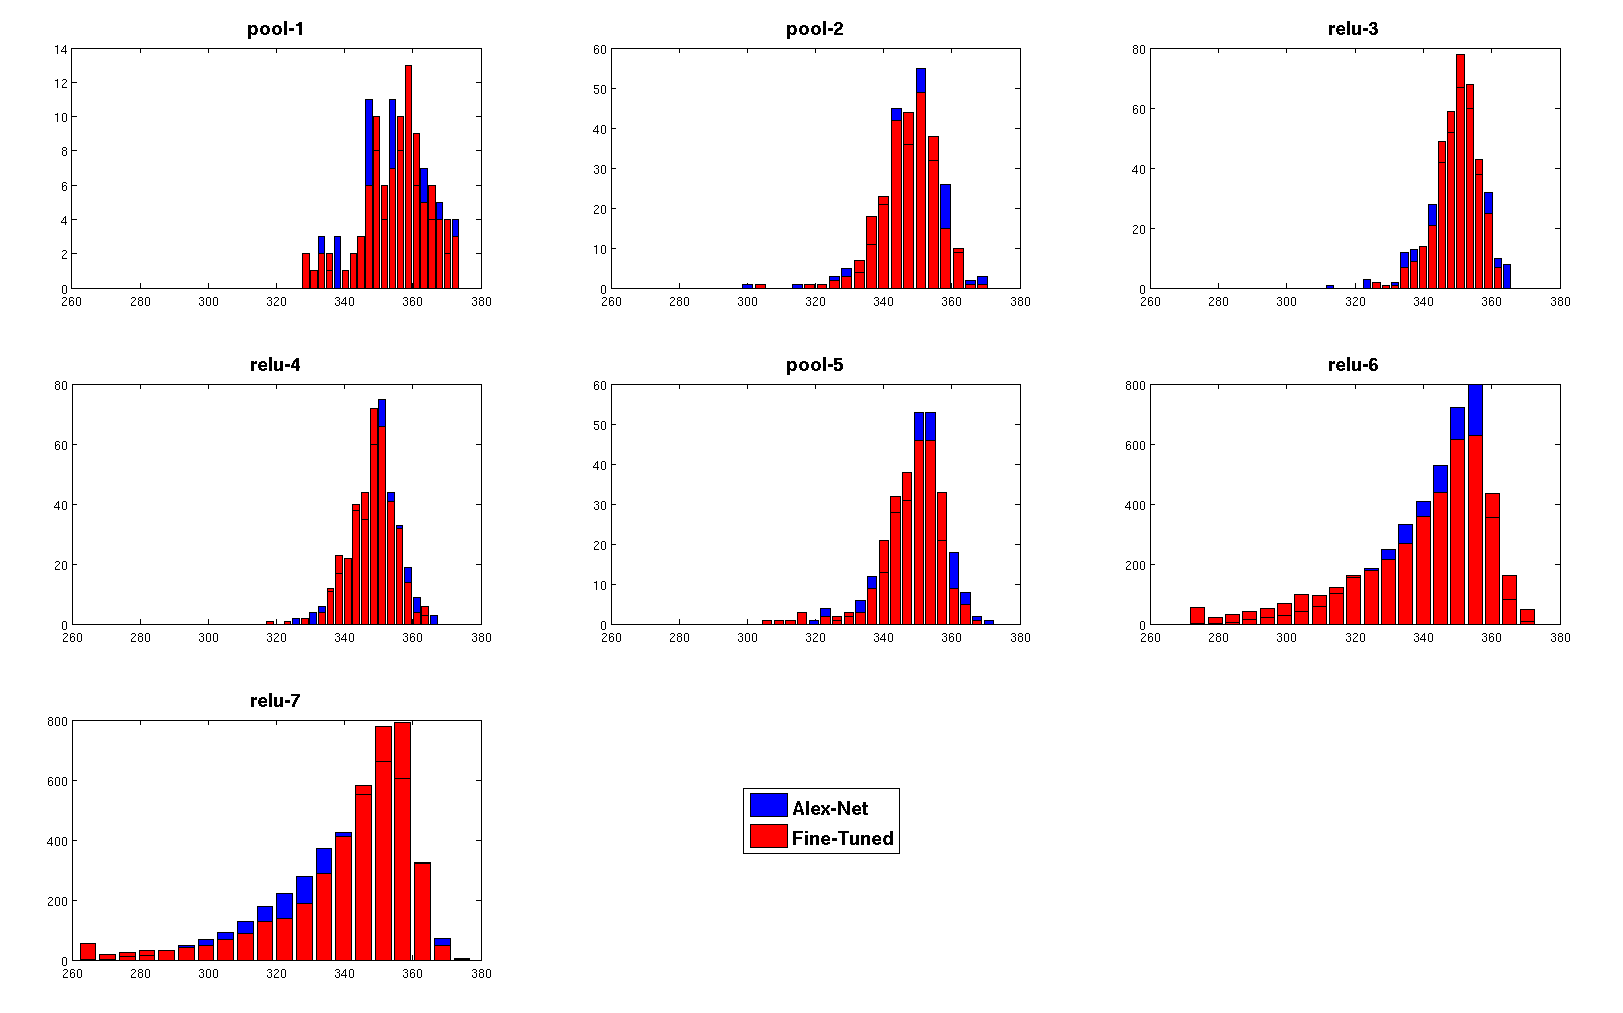
\includegraphics[height=6.5cm]{images/ent_hist.png}}
\caption{Distribution of AuE for different layers in Alex-Net and FT-Net. X-axis is the entropy and the Y-axis is the number of filters. Notice that the left tail for relu 6 and 7 becomes heavier after finetuning. This indicates that finetuning makes these filters more discriminative.}
\label{fig:fine-hist}
\end{figure}

\begin{figure}[t!]
\centering
\subfloat{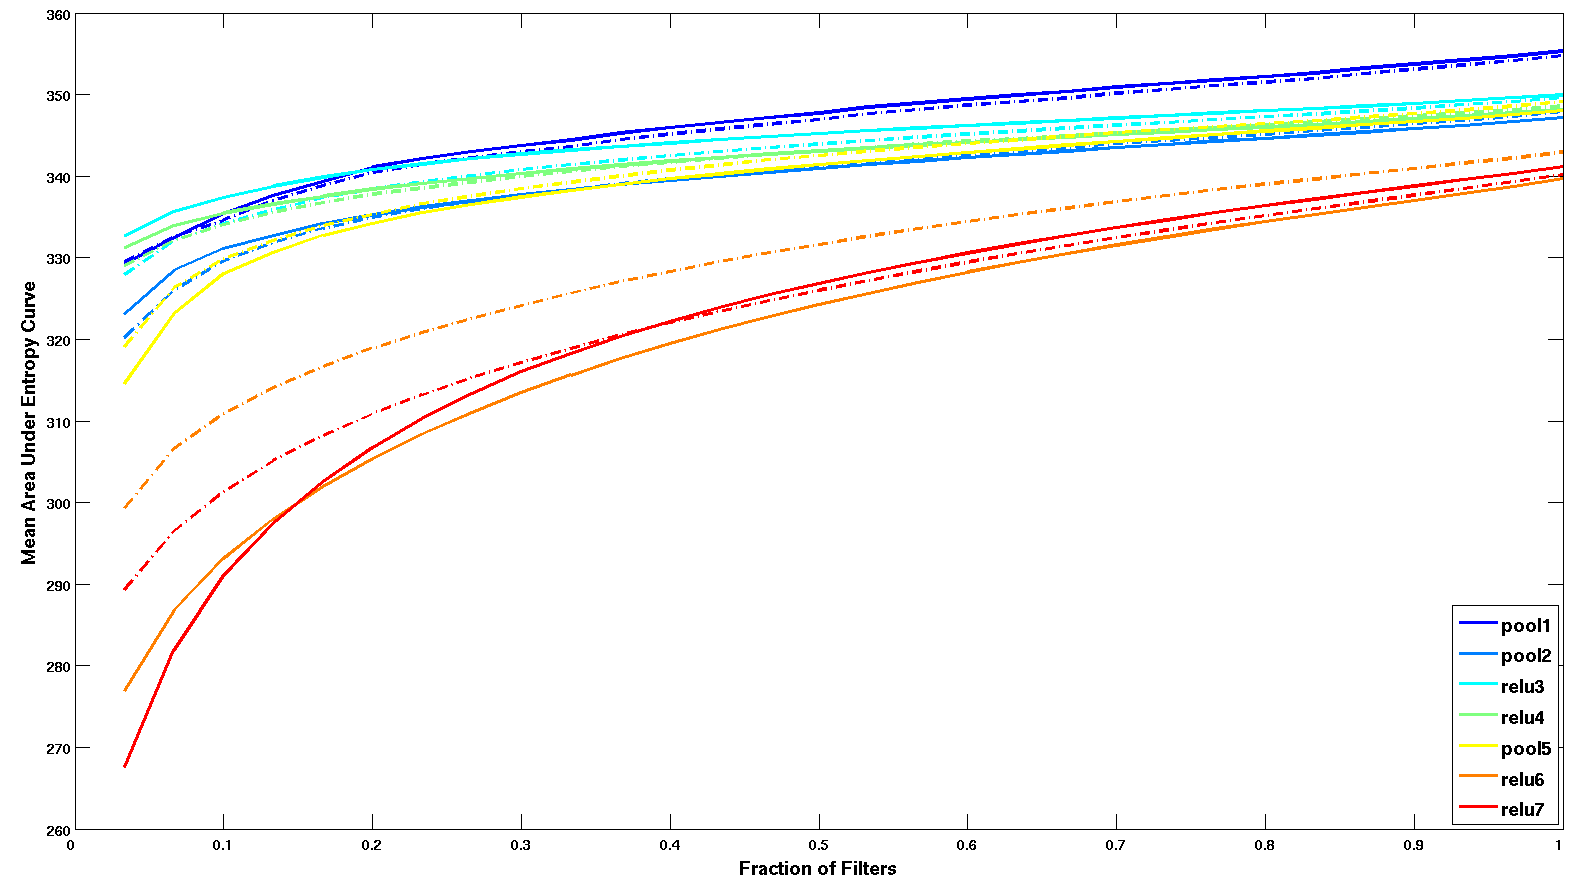
\includegraphics[scale=0.15]{images/entropy_variation.png}}
\caption{Mean Cumulative AuE plotted as fraction of filters (see sec \ref{sub:fine-entropy}). (Dash-Dot Line :Alex-Net, Solid Line: Fine-Tuned Network).}
\label{fig:fine-entropy}
\end{figure}

From figures \ref{fig:fine-hist} and \ref{fig:fine-entropy}, we draw 2 conclusions:
\begin{enumerate}
\item Although the entropy of filters decreases as we move to higher layers, the magnitude of change in entropy between layer 1 and layer 5 is small as compared to the change which happens when going from layer 5 to layer 6.
\item Finetuning mostly reduces the entropy of filters in the fully connected layers, there are small changes in layer 5 and negligible changes in other layers.
\end{enumerate} 

\subsection{Is finetuning only the fully-connected layers sufficient?}
\label{sub:fine-fc-only}
The observations made in \ref{sub:fine-entropy} indicate that finetuning the convolutional layers in the CNN may not be critical for achieving good-performance on novel datasets. We test this hypothesis on the 2 challenging tasks of object detection(PASCAL) and scene classification (SUN-397) by comparing the performance of a fully finetuned network with a network finetuned by only updating weights in the fully-connected (fc) layers. Our results are summarized in table \ref{table:fine-effect}.

\setlength{\tabcolsep}{2pt}
\begin{table}[t!]
\begin{center}
\caption{Comparison in performance on of Alex-Net, Finetuned Network(ft-net) and a network with only fc layers finetuned (fc-ft).}
\label{table:fine-effect}
\scalebox{0.85}{
\begin{tabular}{|l|cccc|cccc|cccc|}
\hline
Layer &  \multicolumn{4}{c|}{sun-397} & \multicolumn{4}{c|}{det VOC-2007-finetune} & \multicolumn{4}{c|}{det VOC-all-finetune} \\
\hline
  &    scratch & i-net & ft & fc-ft  & scratch & i-net & ft & fc-ft & scratch & i-net & ft & fc-ft\\
\hline
fc-7 & $40.2 \pm $ & $53.1 \pm 0.2$ & $56.8 \pm 0.2$ & $56.2 \pm 0.1$ & 40.7 & 45.5 & 54.1 & 53.3 & 52.3 & 53.1 & 56.0 & 59.2 \\ 
\hline
\end{tabular}}
\end{center}
\end{table}
\setlength{\tabcolsep}{1.4pt}

We find that indeed it is the case that the final performance in the detection setup only drops by 0.8 points and by 0.6 points for scene-classification. In our experiments we also noted accuracy of image classification on PASCAL is almost untouched by finetuning. This is suggestive of the fact finetuning is a task specific operation and finetuning for detection does not necessarily leads to an increase in classification performance, even though the classes and images are shared across PASCAL classification and detection challenges. 

\setlength{\tabcolsep}{1pt}
\begin{table}[t!]
\begin{center}
\caption{Evaluation of effect finetuning towards the task of object detection. (l5, l6, l7: layers 5, 6 and 7 of Alex Net)}
\label{table:det-fine}
\scalebox{0.75}{
\begin{tabular}{l|cccccccccccccccccccc||c}
\hline\noalign{\smallskip}
layer & aero & bike & bird & boat & bottle & bus & car & cat & chair & cow & table & dog & horse & mbike & person & plant & sheep & sofa & train & tv & mAP \\
\noalign{\smallskip}
\hline
l5 & 51.9 & 61.1 & 36.8 & 28.4 & 23.7 & 52.3 & 60.8 & 48.4 & 24.9 & 47.1 & 47.5 & 42.1 & 55.6 & 58.7 & 42.5 & 24.5 & 46.9 & 39.3 & 52.0 & 55.4 & 45.0 \\
l5-ft & 57.8 & 63.9 & 38.8 & 28.0 & 29.0&54.8&66.9&51.3 & 30.5 & 52.1 & 45.2 & 43.2 & 57.3 & 58.8 & 46.0 & 27.2 & 51.2 & 39.3 & 53.3 & 56.6 & 47.6 \\
\hline 
l6-ft &63.5 & 66.3 & 48.7 & 38.1 & 30.6 & 61.4 & 70.9 & 60.3 & 34.8 & 57.8 & 47.6 & 53.6 & 59.8 & 63.5 & 52.5 & 29.8 & 54.6 & 48.2 & 58.5 & 62.2 & 53.1 \\
l6-fc-ft& 61.4 & 63.9 & 44.2 & 36.2 & 29.0 & 59.9 & 66.0 & 55.3 & 31.1 & 57.6 & 49.5 & 49.4 & 59.4 & 63.7 & 50.8 & 29.5 & 54.1 & 43.2 & 57.4 & 58.8 & 51.0 \\
\hline
l7 & 57.6 & 57.2 & 41.4 & 31.2 & 25.6 & 52.4 & 58.8 & 50.9 & 25.2 & 50.4 & 42.7 & 47.1 & 52.2 & 55.6 & 44.5 & 23.9 & 48.0 & 38.1 & 51.5 & 56.6 & 45.5 \\
l7-ft & 64.3 & 69.6 & 50.1 & 41.8 & 32.0 & 62.6 & 71.0 & 60.6 & 32.8 & 58.5 & 46.4 & 56.0 & 60.0 & 66.9 & 54.2 & 31.5 & 52.7 & 48.8 & 57.7 & 64.7 & 54.1 \\
l7-fc-ft & 62.9 & 65.2 & 47.5 & 39.0 & 30.3 & 63.1 & 68.4 & 59.7 & 34.2 & 58.5 & 52.0 & 53.8 & 60.7 & 65.3 & 53.0 & 30.2 & 55.5 & 46.3 & 57.7 & 62.2 & 53.3 \\
\hline
\end{tabular}}
\end{center}
\end{table}
\setlength{\tabcolsep}{1.4pt}

A detailed layer-wise analysis of detection performance for all PASCAL classes and the 3 network configurations is presented in table \ref{table:det-fine}. Notice that for both the finetuned networks there is big jump in the performance while going from layer 5 to 6 and a rather small jump from layer 6 to 7. For Alex-Net, the performance is virtually the same for layers 5 and 7. It is also notable, that although the performance for FT-net is better by 2.6 points at layer 5 - the performance is virtually the same at layer 7. 
\subsection{Discussion}
\label{sub:fine-discussion}
Since layers 1-5 change a little over the course finetuning, this suggests that these are generic features. Although, one could always improve performance by a few points by finetuning the full network - for a lot of applications this may not be practical. 
It is also notable to point out that the more or less generic representations learnt in layer 4 and 5 are in contrast with some of the mid-level feature learning work such as \cite{Blocks} \cite{Mid1} wherein the problem of finding good mid-level parts is often posed as a greedy search for high recall discriminative templates.

\section{How do the different layers of a CNN train over time? How much pretraining is sufficient?}
\label{sec:speed}
Training CNNs is very time consuming. \cite{Kriz} trained for around 7 days for achieving state of art results on Imagenet. Even finetuning for PASCAL object detection \cite{Rcnn} takes over 12 hours on the advanced GPUs such as the Nvidia Tesla-K40. This is a big barrier towards exploring different network architectures. Layerwise training has been previously used for learning parameters of multilayer networks(REF). We hypothesized, that maybe such methods which train one layer at a time can be used to speed-up CNN training. Before, testing this we sought to determine if simultaneous learning of parameters in all layers of CNNs by itself proceeds in a layerwise manner. 

We started our analysis by studying the evolution of training loss and validation accuracy of a CNN trained for Imagenet classification (see fig \ref{fig:conv1}). The top-1 accuracy on the validation set after 15K iterations is at 29.5 \% and 38.13\% after 50K  iterations (compared to 57.4 \% at 310K iterations). The training loss rapidly increases initially and then there is a slow sluggish decay except at time points where learning rate is decimated by a factor of 10 after every 100K iterations. Such a behaviour is reminiscent of stochastic gradient descent(NEED REF) and is not surprising. 

\begin{figure}[t!]
\centering
\subfloat[Validation Set Accuracy (Red) and Training Loss (Blue)]{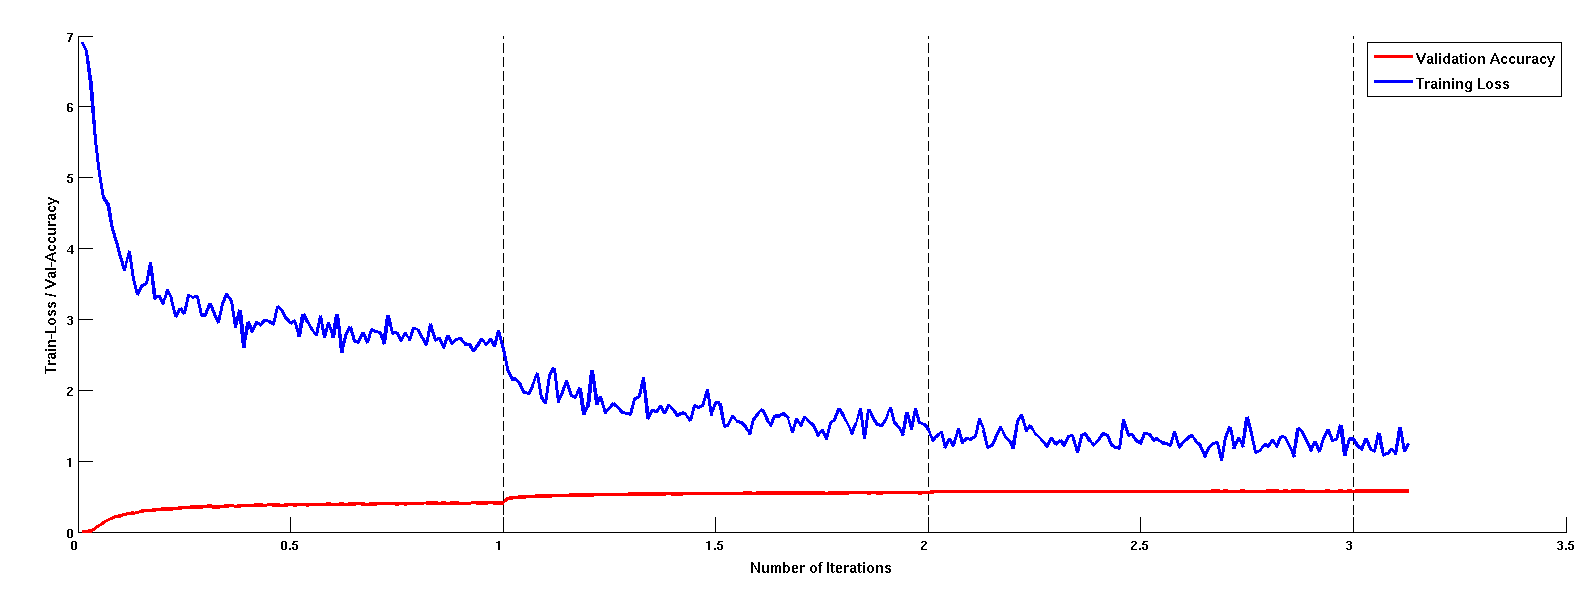
\includegraphics[scale=0.15]{images/training_loss.png}}\\
\subfloat[5K Iterations]{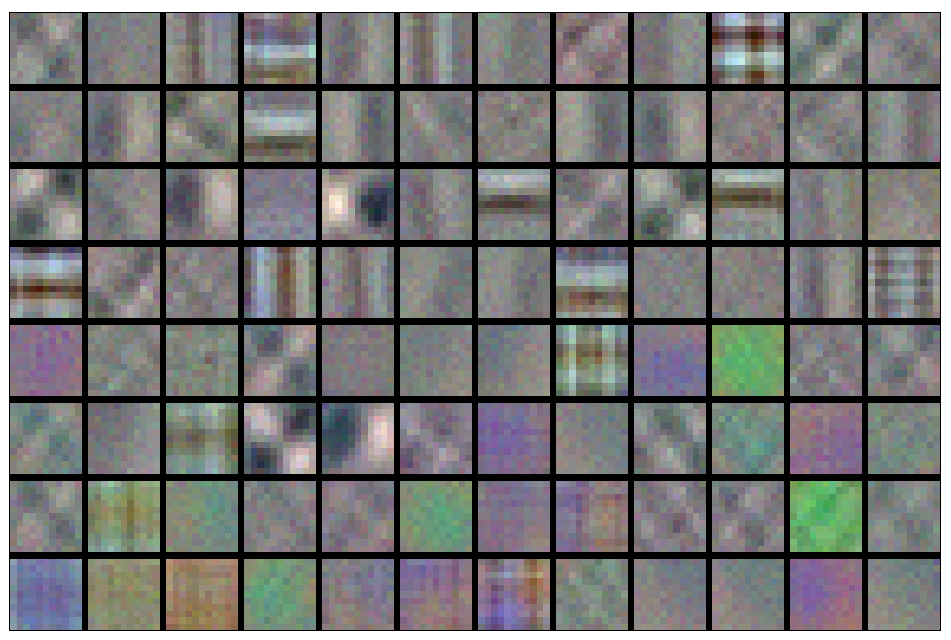
\includegraphics[scale=0.10]{images/l1_filters_iter5000.png}} \hspace{2mm}
\subfloat[15K Iterations]{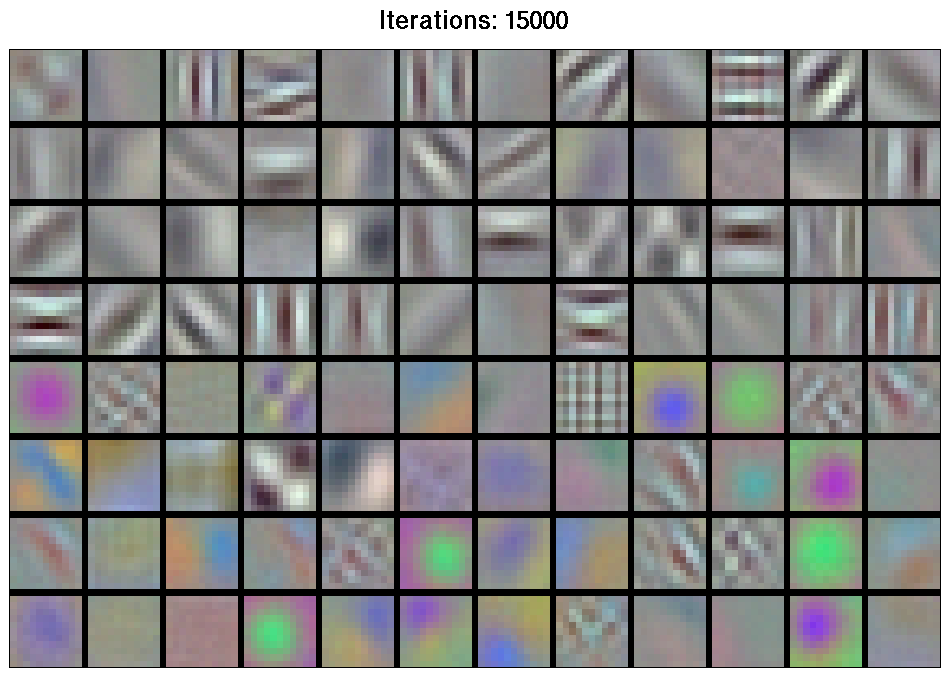
\includegraphics[scale=0.10]{images/l1_filters_iter15000.png}} \hspace{2mm}
\subfloat[225K Iterations]{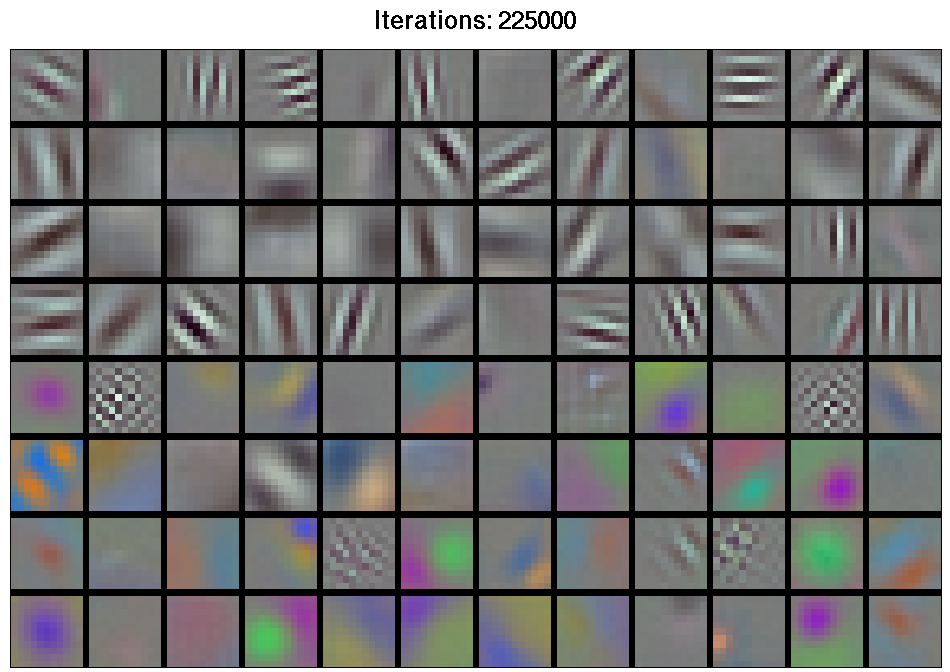
\includegraphics[scale=0.10]{images/l1_filters_iter225000.png}}
\caption{(a) shows the evolution of top-1 accuracy on the validation set (red) and training loss (blue) as a function of number of iterations. The vertical dotted black lines are the time points when the learning rate is reduced by a factor of 10. It can be seen, that the accuracy improves substantially when the learning rate is reduced. (b),(c),(d) show conv-1 filters after 5K, 15K and 225K iterations of training respectively. One pass (epoch) over the entire Imagenet-ILSVRC12 dataset takes approximately 5K iterations. Notice, that just after 15K iterations these filters closely resemble their final state.}
\label{fig:conv1}
\end{figure}

For a better understanding. we evaluated performance of a linear svm classifier learned on features extracted from individual layers on Pascal 2007 classification challenge. The results are summarized in table \ref{table:det-traj-classify}.It is quite surprising to note that by 15K iterations all layers are within 80\% and at 50K iterations within 90\% of there final performance. This strongly indicates that a great portion of training required for generalization happens quite quickly. 

\setlength{\tabcolsep}{4pt}
\begin{table}[t!]
\begin{center}
\caption{Variation in classification accuracy (mean-AP) on PASCAL VOC 2007 challenge using features extracted from different layers of Alex-Net as a function of number of iterations.}
\label{table:det-traj-classify}
\begin{tabular}{lcccccccc}
\hline\noalign{\smallskip}
Layer  & 5K & 15K & 25K & 35K & 45K & 95K & 105K & 310K \\
\noalign{\smallskip}
\hline
\noalign{\smallskip}
conv-1 & 23.0 & 24.3 & 24.4 & 24.5 & 24.6 & 24.8 & 24.7 & 25.1\\
conv-2 & 33.7 & 40.4 & 40.9 & 41.8 & 42.0 & 43.2 & 44.0 & 45.0\\
conv-3 & 34.2 & 46.8 & 47.0 & 48.2 & 48.5 & 49.4 & 51.6 & 50.1\\
conv-4 & 33.5 & 49.0 & 48.7 & 50.2 & 50.6 & 51.6 & 54.1 & 54.2\\
conv-5 & 33.0 & 53.4 & 55.0 & 56.8 & 57.4 & 59.2 & 63.5 & 65.6\\
fc-6 & 34.2 & 59.7 & 62.6 & 62.7 & 64.1 & 65.6 & 69.3 & 70.6\\
fc-7 & 30.9 & 61.3 & 64.1 & 65.1 & 65.8 & 67.8 & 71.8 & 73.2\\
\hline
\end{tabular}
\end{center}
\end{table}
\setlength{\tabcolsep}{1.4pt}

Motivated by these observations we trained a 50-50 network (50K iterations on imagenet and finetuned for 50K iterations using the procedure described in sec. \ref{sub:fine-train}) and evaluated its performance on the  Pascal 2007 detection challenge (see table \ref{table:det-trajectory} for results). Consistent with our earlier results we find that this network achieves a surprising performance of 48.6 mean AP points compared to 54.1 achieved by pre-training for 310K iterations. 

\setlength{\tabcolsep}{1pt}
\begin{table}[t!]
\begin{center}
\caption{Performance of 50-50 network for detection on pascal-voc-2007 challenge. (l5 is conv-5 and l7 is fc-7)}
\label{table:det-trajectory}
\scalebox{0.70}{
\begin{tabular}{l|cccccccccccccccccccc||c}
\hline\noalign{\smallskip}
Feature & aero & bike & bird & boat & bottle & bus & car & cat & chair & cow & table & dog & horse & mbike & person & plant & sheep & sofa & train & tv & mAP \\
\noalign{\smallskip}
\hline
l5(50-50) & 55.2 & 58.4 & 31.0 & 28.8 & 21.0 & 53.5 & 63.6 & 41.0 & 25.4 & 44.7 & 40.9 & 34.9 & 49.5 & 56.9 & 43.8 & 25.2 & 45.3 & 31.2 & 48.7 & 54.4 & 42.7 \\
l5 (full) & 57.8 & 63.9 & 38.8 & 28.0 & 29.0&54.8&66.9&51.3 & 30.5 & 52.1 & 45.2 & 43.2 & 57.3 & 58.8 & 46.0 & 27.2 & 51.2 & 39.3 & 53.3 & 56.6 & 47.6 \\
\hline
l7(50-50) & 58.7 & 64.8 & 38.2 & 34.9 & 25.9 & 59.5 & 69.5 & 46.2 & 28.7 & 52.4 & 45.2 & 44.3 & 57.3 & 63.4 & 52.4 & 28.0 & 51.5 & 34.9 & 56.0 & 59.4 & 48.6 \\
l7(full) & 64.3 & 69.6 & 50.1 & 41.8 & 32.0 & 62.6 & 71.0 & 60.6 & 32.8 & 58.5 & 46.4 & 56.0 & 60.0 & 66.9 & 54.2 & 31.5 & 52.7 & 48.8 & 57.7 & 64.7 & 54.1 \\
\hline
\end{tabular}}
\end{center}
\end{table}
\setlength{\tabcolsep}{1.4pt}
The above analysis reinforces our belief that indeed majority of training required for generalization happens quite quickly as compared to the full training time of the network. This observation suggest that there may exist clever ways which can help us speed up the training.



\section{Conclusion}
\label{sec:conclusion}
In this paper we analysed different properties of convolutional neural networks with the aim of gaining insights required to efficiently exploit the rich feature hierarchies provided by such networks. \\

\noindent \textbf{Acknowledgements}

\begin{align}
  \psi (u) & = \int_{0}^{T} \left[\frac{1}{2}
  \left(\Lambda_{0}^{-1} u,u\right) + N^{\ast} (-u)\right] dt \; \\
& = 0 ?
\end{align}


\bibliographystyle{splncs03}
\bibliography{egbib}
\end{document}
